\section{N-gram prediction}
\label{sec:n_gram}

As mentioned in sections \ref{sec:information_and_entropy} and \ref{sec:regularity_and_context}, the entropy of a single letter in English is 4.14 bits, but that is when the letter is considered out of context.

In his paper "Prediction and entropy of printed English" \textcite{Shannon1951} checks the effect of context by giving subjects a varying amount of context from a text (1 to 100 previous letters) and asking them to guess the next letter, keeping track of how often the first guess, second guess, etc. is correct. In the case where subjects were given 100 previous letters, they guess accurately on their first try 80\% of the time and on their second try 7\% of the time. After some analysis, he estimates that - when a letter is considered within its context - English contains 0.6 to 1.3 bits of information per letter.

To check this value, I apply the method of analysis given in the 1951 paper using modern tools.

The method considers n-grams (groups of $n$ consecutive characters) in a text and defines the entropy of n-grams in English as

$$G_n = -\sum_{b \in B_n} p(b) \log p(b)$$

where $B_n$ is the set of all possible n-grams and $p(b)$ is the frequency with which the n-gram $b$ occurs in English text. For example, $G_1 = p('e') \log p('e') + p('t') \log p('t') + ...$ = 4.14 is the entropy of 1-grams, that is, single letters.

Building on this, Shannon evaluates the average entropy of the last character in the n-gram given the previous $n-1$ characters. This is

\begin{align*}
F_n &= && \sum_{r \in B_{n-1}} p(r) (\text{entropy of the last character } c \text{ given the prefix } r) \\
&= && \sum_{r \in B_{n-1}} p(r) (-\sum_{c \in C} p(c|r) \log p(c|r)) \\
&= &- & \sum_{r \in B_{n-1},  c \in C} p(r,c) \log p(c|r) \\
&= &- & \sum_{r \in B_{n-1},  c \in C} p(r,c) \log p(r,c) +  \sum_{r \in B_{n-1},  c \in C} p(r,c) \log p(r) \\
&= &- & \sum_{b \in B_n} p(b) \log p(b) + \sum_{b \in B_{n-1}} p(b) \log p(b) \\
&= && G_n - G_{n-1} 
\end{align*}


$F_n$ is the differential or marginal entropy at the last letter of an N-gram, that is, how much uncertainty there is about that letter when the previous $n-1$ letters are known, and correspondingly how much information it carries.

To estimate the values of $G_n$ and $F_n$ for various $n$, I concatenate all texts from the Gutenberg dataset and use python's \texttt{Counter} tool to track how many times each n-gram occurs. The counts of n-grams are then used to calculate the n-gram entropies $G_n$ and their differences give the values of $F_n$, The results are shown in tables \ref{tab:n_gram_entropy} and \ref{tab:n_word_entropy}.


\begin{table}[h]
\centering
\begin{tabular}{ |p{1cm}||p{3cm}|p{3cm}|  }
 %\hline
 %\multicolumn{3}{|c|}{Compression algorithm benchmarks} \\
 \hline
    N  & N-gram entropy & Marginal entropy\\
 \hline
    1  &     4.668763   &    4.668763\\
    2  &     8.174800   &    3.506037\\
    3  &    11.028968   &    2.854169\\
    4  &    13.345969   &    2.317001\\
    5  &    15.323687   &    1.977718\\
    6  &    17.094342   &    1.770655\\
    7  &    18.704355   &    1.610013\\
    8  &    20.150312   &    1.445958\\
    9  &    21.415078   &    1.264766\\
    10 &    22.484581   &    1.069503\\
 \hline
\end{tabular}
\caption{Entropies and marginal entropies for substrings which are $n$ characters long
\label{tab:n_gram_entropy}}
\end{table}



\begin{table}[h]
\centering
\begin{tabular}{ |p{1cm}||p{3cm}|p{3cm}|  }
 %\hline
 %\multicolumn{3}{|c|}{Compression algorithm benchmarks} \\
 \hline
    N  & N-gram entropy & Marginal entropy\\
 \hline
    1  &    11.348724   &     11.348724\\
    2  &    18.610973   &      7.262249\\
    3  &    22.132126   &      3.521153\\
    4  &    23.172127   &      1.040001\\
 \hline
\end{tabular}
\caption{Entropies and marginal entropies for substrings which are $n$ words long
\label{tab:n_word_entropy}}
\end{table}

Table \ref{tab:n_gram_entropy} shows the entropies for substrings of the text which are $n$ letters long, along with the marginal entropy at the last letter, conditional on knowledge of the previous $n-1$ letters, while table \ref{tab:n_word_entropy} shows entropies for substrings which are $n$ words long, along with the marginal entropy at the last word.

As can be seen in both tables, more knowledge about the context in which a letter or word appears decreases the information content and increases the predictability of that letter or word.

For example, the entry $1.04$ on the fourth line of table \ref{tab:n_word_entropy} indicates that when three consecutive words of a text are known, the fourth word contains approximately 1 bit of information, that is, there are on average only two candidates for what the fourth word could be.

The data displayed in table \ref{tab:n_gram_entropy} empirically validates the estimate of 0.6-1.3 bits per letter. As English text is often encoded in 1 byte per letter, this indicates an ideal compression ratio (ratio of uncompressed text size to compressed text size) of approximately 8.


\subsection{Practical application}

Next, I examine Shannon's concept of the Ideal N-gram Predictor, which he conceptualizes as a lookup table with the keys being the set of all possible [n-1]-grams and the values being an ordering of all possible following symbols ranked by their likelihood. For example, a 3-gram predictor would have among its keys the 2-gram "qu" and in the value corresponding to that key all possible following letters starting with "e" and going down in terms of likelihood (as "que" is the most common 3-gram in English text that starts with "qu").

In the original formulation, a text is compressed for transmission by replacing each letter in it with its rank given the previous [n-1]-gram. For example, the word "queue" may be transmitted as the numbers 15,1,1,1,1, indicating that "q" was the 15th most likely letter at the start of a text, "u" was the 1st most likely letter to follow, etc.

I test the practical application of this idea by using Huffman and arithmetic codes instead of integers, assigning the most likely symbols (within a given context) the shortest codes, and check to see how well these implementations perform in terms of compression ratio. To do this, I create the following classes in my code

\begin{itemize}
  \item A \texttt{Code} superclass, subclassed by the \texttt{Huffman} and \texttt{Arithmetic} classes, each of which handles the construction of a code given the probabilities of the symbols, as well as handle encoding and decoding of symbols.
  \item A \texttt{Predictor} abstract class, subclassed by \texttt{NGramPredictor} (and in section \ref{sec:machine_learning} by \texttt{LSTMPredictor} and \texttt{RNNPredictor} as well). \texttt{Predictor} objects must have a \texttt{train()} method which trains the predictor on a basis text from which it detects the regularities in the language and a \texttt{probabilities\_given\_context()} method which takes a context as its input and outputs a mapping of symbols to their probabilities within that context.
  \item A \texttt{Compressor} class. Objects of this class are initialized with a \texttt{Predictor} and a \texttt{Code} object, and provide \texttt{encode()} and \texttt{decode()} methods, leveraging its associated \texttt{Predictor} to estimate the probabilities of symbols within a given context, and its associated \texttt{Code} to generate the corresponding entropy coding for that context and encode/decode the input text.
\end{itemize}

In particular, the \texttt{NGramPredictor} class is initialized with
\begin{itemize}
  \item A basis text from which the predictor infers the patterns of the language of the text (and which it is trained on immediately)
  \item A window size. This sets the value of $n$ for which it will examine n-grams in the text. For example, a window size of 6 means that the predictor will construct a lookup table mapping 5-grams and to the probabilities of different symbols being the completion of that 5-gram into a 6-gram.
\end{itemize}

The code for the libraries I create for this task can be found at \texttt{\href{https://github.com/Guy29/FYP/blob/main/Code/libraries}{Code/libraries}} and an application of them at \texttt{\href{https://github.com/Guy29/FYP/blob/main/Code/n_gram}{Code/n\_gram}}. In the first, I implement the \texttt{Huffman} and \texttt{Arithmetic} classes from scratch. I initially considered using functions defined in the python library \texttt{bitarray} for Huffman codes (namely \texttt{decodetree} and \texttt{huffman\_code}), but opted not to as these did not provide all the functionalities I wanted and did not conform to the desired interface. Through some experimentation, it also seems that my implementation is faster to run that \texttt{bitarray}'s.

To test my code, I begin by creating a \texttt{Predictor} object trained on War and Peace with a window size of 6, and from it create the corresponding \texttt{Compressor} object (I will refer to this as WPC). I then use WPC to encode and decode simple phrases to ensure that the operations reverse correctly. The \texttt{encode} method takes a sequence of bytes (ideally in natural language) and compresses them using the lookup table constructed from the 6-grams found in War and Peace. Figure \ref{fig:inigo_encoding_decoding} illustrates a simple use case.

\begin{figure}[h]
\centering
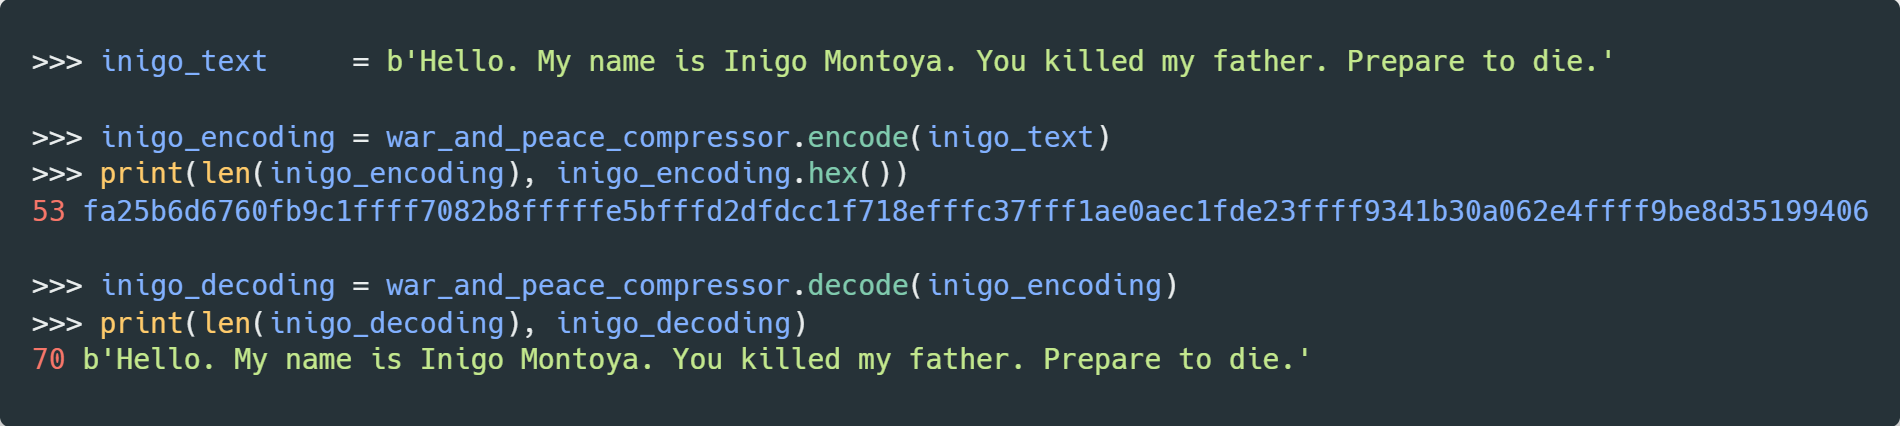
\includegraphics[width=\textwidth]{img/inigo_encoding_decoding.png}
\caption{Using WPC to encode and decode a few sentences.}
\label{fig:inigo_encoding_decoding}
\end{figure}

It is also possible to use the \texttt{decode} method on randomly generated bytes to obtain text that follows the regularities which the predictor has learned, as in figure \ref{fig:predictor_decoding_randomness}.

\begin{figure}[h]
\centering
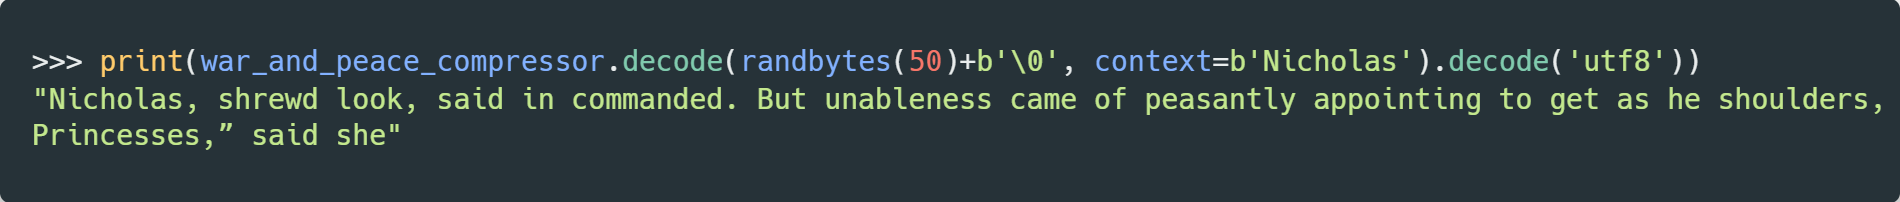
\includegraphics[width=\textwidth]{img/predictor_decoding_randomness.png}
\caption{Using the \texttt{decode} method on a randomly generated input}
\label{fig:predictor_decoding_randomness}
\end{figure}

The performance of a \texttt{Predictor} object depends on the text it has been trained on, and words and expressions which it is familiar with would therefore have shorter representations in its output encoding. For example, figure \ref{fig:predictor_surprisal_by_char} shows the surprisal of \texttt{war\_and\_peace\_predictor} when trying to predict the characters in the first paragraph of The Adventures of Sherlock Holmes.

\begin{figure}[h!]
\centering
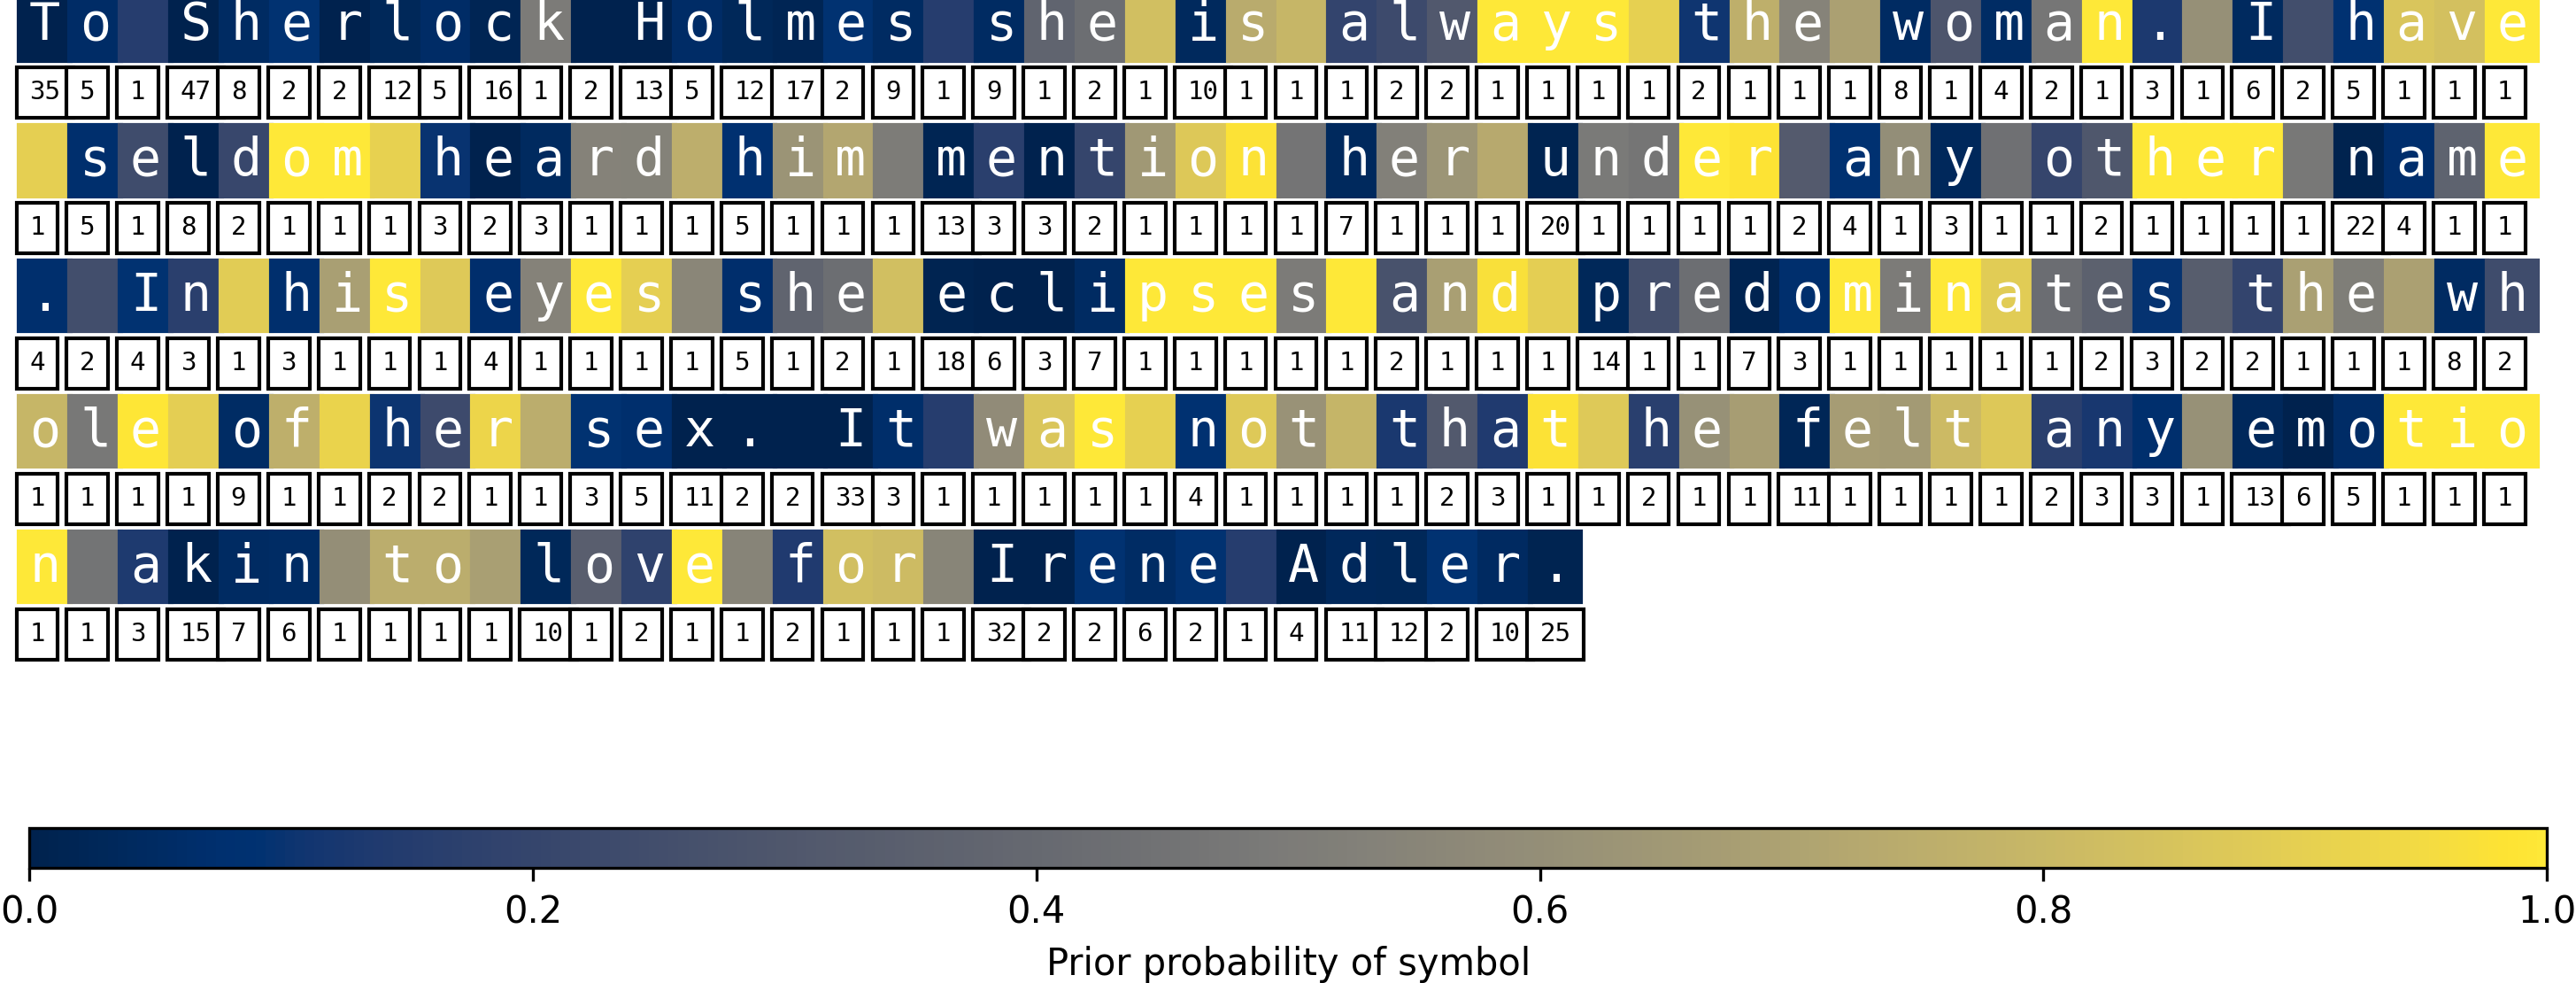
\includegraphics[width=\textwidth]{img/predictor_surprisal_by_char.png}
\caption{Surprisal of the \texttt{war\_and\_peace\_predictor} at each symbol in the opening passage of Sherlock Holmes. The prior probability given by the model to each symbol is indicated by its color, while how highly it ranked this symbol in terms of probability is indicated by a number below the symbol.}
\label{fig:predictor_surprisal_by_char}
\end{figure}

A few observations on figure \ref{fig:predictor_surprisal_by_char},

\begin{itemize}
    \item For the first few symbols, the predictor performs badly as it has no context from which to infer the next symbol.
    \item The predictor performs especially badly for proper nouns. This is to be expected, as the words "Sherlock Holmes" and "Irene Adler" are not ones which it would have come across in War and Peace.
    \item The letter "k" at the end of "Sherlock" was expected with 0.5 probability by the model. On further investigation it seems this is because the 5-gram "erloc" appears in W\&P twice, in the words "interlocutor" and "interlocking", and half of these have a "k" following "erloc".
    \item The predictor often performs better on the ending of words than their beginning.
    \item For commonly found phrases such as "was not that he", the predictor's first guess for the following letter is very often correct.
\end{itemize}

Figure \ref{fig:predictor_surprisal_by_char} gives the probability rank of each symbol underneath it. For example, a rank of 2 indicates that the symbol would have been the predictor's second guess based on the previous 5-gram.

Figure \ref{fig:predictor_surprisal_histogram} and table \ref{tab:predictor_surprisal} show the rank distribution when encoding the entire text of The Adventures of Sherlock Holmes.

\begin{figure}[h]
\centering
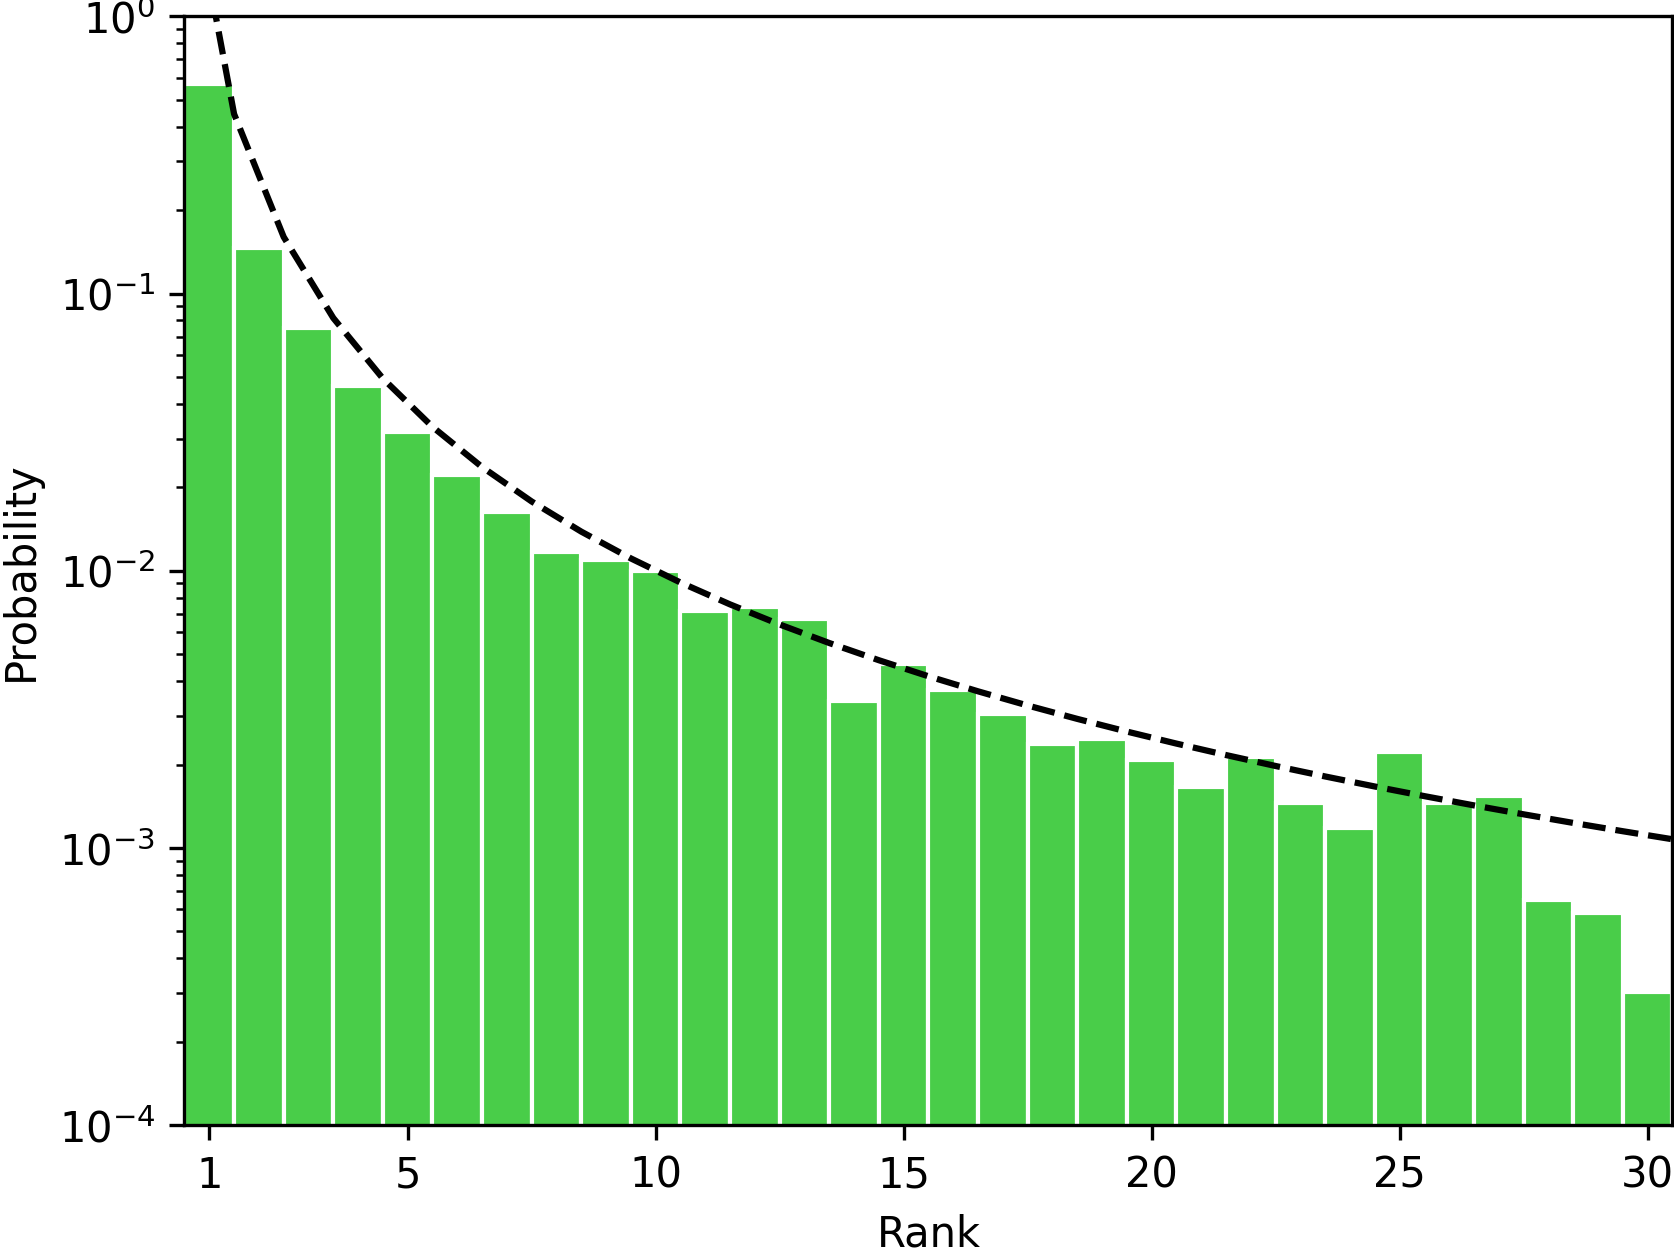
\includegraphics[width=\textwidth]{img/predictor_surprisal_histogram.png}
\caption{In this histogram, each bin represents a symbol rank from 1 to 30, and the height of the bin represents the frequency at which this rank occurs in the WPC's encoding of The Adventures of Sherlock Holmes. The dashed line shows the probability density function for the Pareto distribution with a scale of 1 and a shape of 1.}
\label{fig:predictor_surprisal_histogram}
\end{figure}

\begin{table}[ht]
\centering
\begin{tabular}{ |p{4cm}||p{1.5cm}|p{1.5cm}|p{1.5cm}|p{1.5cm}|p{1.5cm}|  }
 \hline
    Rank & 1 & 2 & 3 & 4 & 5\\
 \hline
    Probability & 0.568561 & 0.146148 & 0.075059 & 0.046406 & 0.031536\\
 \hline
    Human performance & 0.58 & 0.19 & 0.05 & 0.01 & 0.04\\
 \hline
    Zeta distribution ($6/{{\pi^2}{r^2}}$) & 0.607927 & 0.151982 & 0.067547 & 0.037995 & 0.024317\\
 \hline
\end{tabular}
\caption{In the first row, this table shows how often the WPC is correct in its first guess, second guess, etc. for the last letter in a 6-gram. The second row gives values given by \textcite{Shannon1951} obtained through experiments with English speakers similarly given 5 letters of context and asked to predict the full 6-gram. The third row gives the values of the zeta distribution with parameter 2 for comparison.}
\label{tab:predictor_surprisal}
\end{table}


The predictor trained on War and Peace accurately predicts a symbol based on the previous 5-gram on its first try 56.86\% of the time, and the frequency of the ranks follows a Pareto distribution with a scale parameter of 1 and a shape parameter of 1, i.e. the probability density function is $1/r^2$. The values for the discrete version of this distribution (the zeta distribution with parameter 2) is included in table \ref{tab:predictor_surprisal} for comparison.

When initializing a \texttt{Compressor} object, one has a choice between using Huffman coding or arithmetic coding (by passing either the \texttt{Huffman} or the \texttt{Arithmetic} class as a parameter). These differ in how they assign binary codes to symbols, with Huffman coding being more economical - the average code length being usually minimal - and arithmetic coding being "fairer", in the sense that a symbol with $2^{-n}$ probability of occurring would have a code that is approximately $n$ bits long, that is, it preserves the probability distribution of the symbols.

For example, if symbol "a" occurs with probability 0.9 and symbol "b" appears with probability 0.1, Huffman coding would assign them the codes "0" and "1" respectively, while arithmetic coding would assign them "0" and "11101". Because of this difference, decoding a random sequence of bits using the Huffman code would result in an output which has an equal number of "a"s and "b"s, whereas decoding the same input using the arithmetic code would result in an output that is approximately 90\% "a"s and 10\% "b"s per the original distribution.

Table \ref{tab:6WPP_performance} shows the performance of WPC on some input texts using each code. For all examined texts (including Don Quixote, which is not in English), the compressed version is no larger than the original, and in fact this method typically performs better than gzip and zlib (see table \ref{tab:compalg_benchmarks}). As expected, Huffman coding yields significantly better results than arithmetic coding. Note also that (apart from its own basis text), WPC performs best on the text of Crime and Punishment, which is the text that is closest to it historically and geographically, and which is therefore likely to contain many of the same regularities.

\begin{table}[h!]
\centering
\begin{tabular}{|l|c|c|}
 \hline
    Text & \makecell{Huffman\\compression ratio} & \makecell{Arithmetic\\compression ratio}\\
 \hline
    War and Peace                             &  4.258278  &  3.404772\\
    Crime and Punishment                      &  3.019220  &  2.068427\\
    Alice's Adventures in Wonderland          &  2.946588  &  2.028157\\
    Middlemarch                               &  2.895632  &  1.950565\\
    The Count of Monte Cristo                 &  2.894389  &  1.947010\\
    Don Quixote                               &  2.715589  &  1.833225\\
    The King James Version of the Bible       &  2.284923  &  1.543722\\
    The Complete Works of William Shakespeare &  1.984536  &  1.289506\\
 \hline
\end{tabular}
\caption{\label{tab:6WPP_performance}}
\end{table}

\subsection{Conclusions and future work}

\todo[inline, color=yellow]{Mention: Shannon tries doing prediction backwards and it works pretty well. This is possible with the `Predictor` class. Is it possible to combine both forwards and backwards prediction?}
\todo[inline, color=yellow]{Mention the potential application of the context given to `Predictor` objects not being previous characters, instead being an indicator of topic or part of speech for example}
\todo[inline, color=yellow]{Mention confabulation}
\todo[inline, color=yellow]{Compare found zeta distribution to Zipf's law. Why should the parameter be approximately 2 for a 6-gram? What's the general law here?}